\sectionframe{Feature Distribution Smoothing (FDS)}

\begin{frame}{Feature statistics similarity for anchor age 0}
	\begin{figure}[h]
		\begin{subfigure}{0.48\textwidth}
			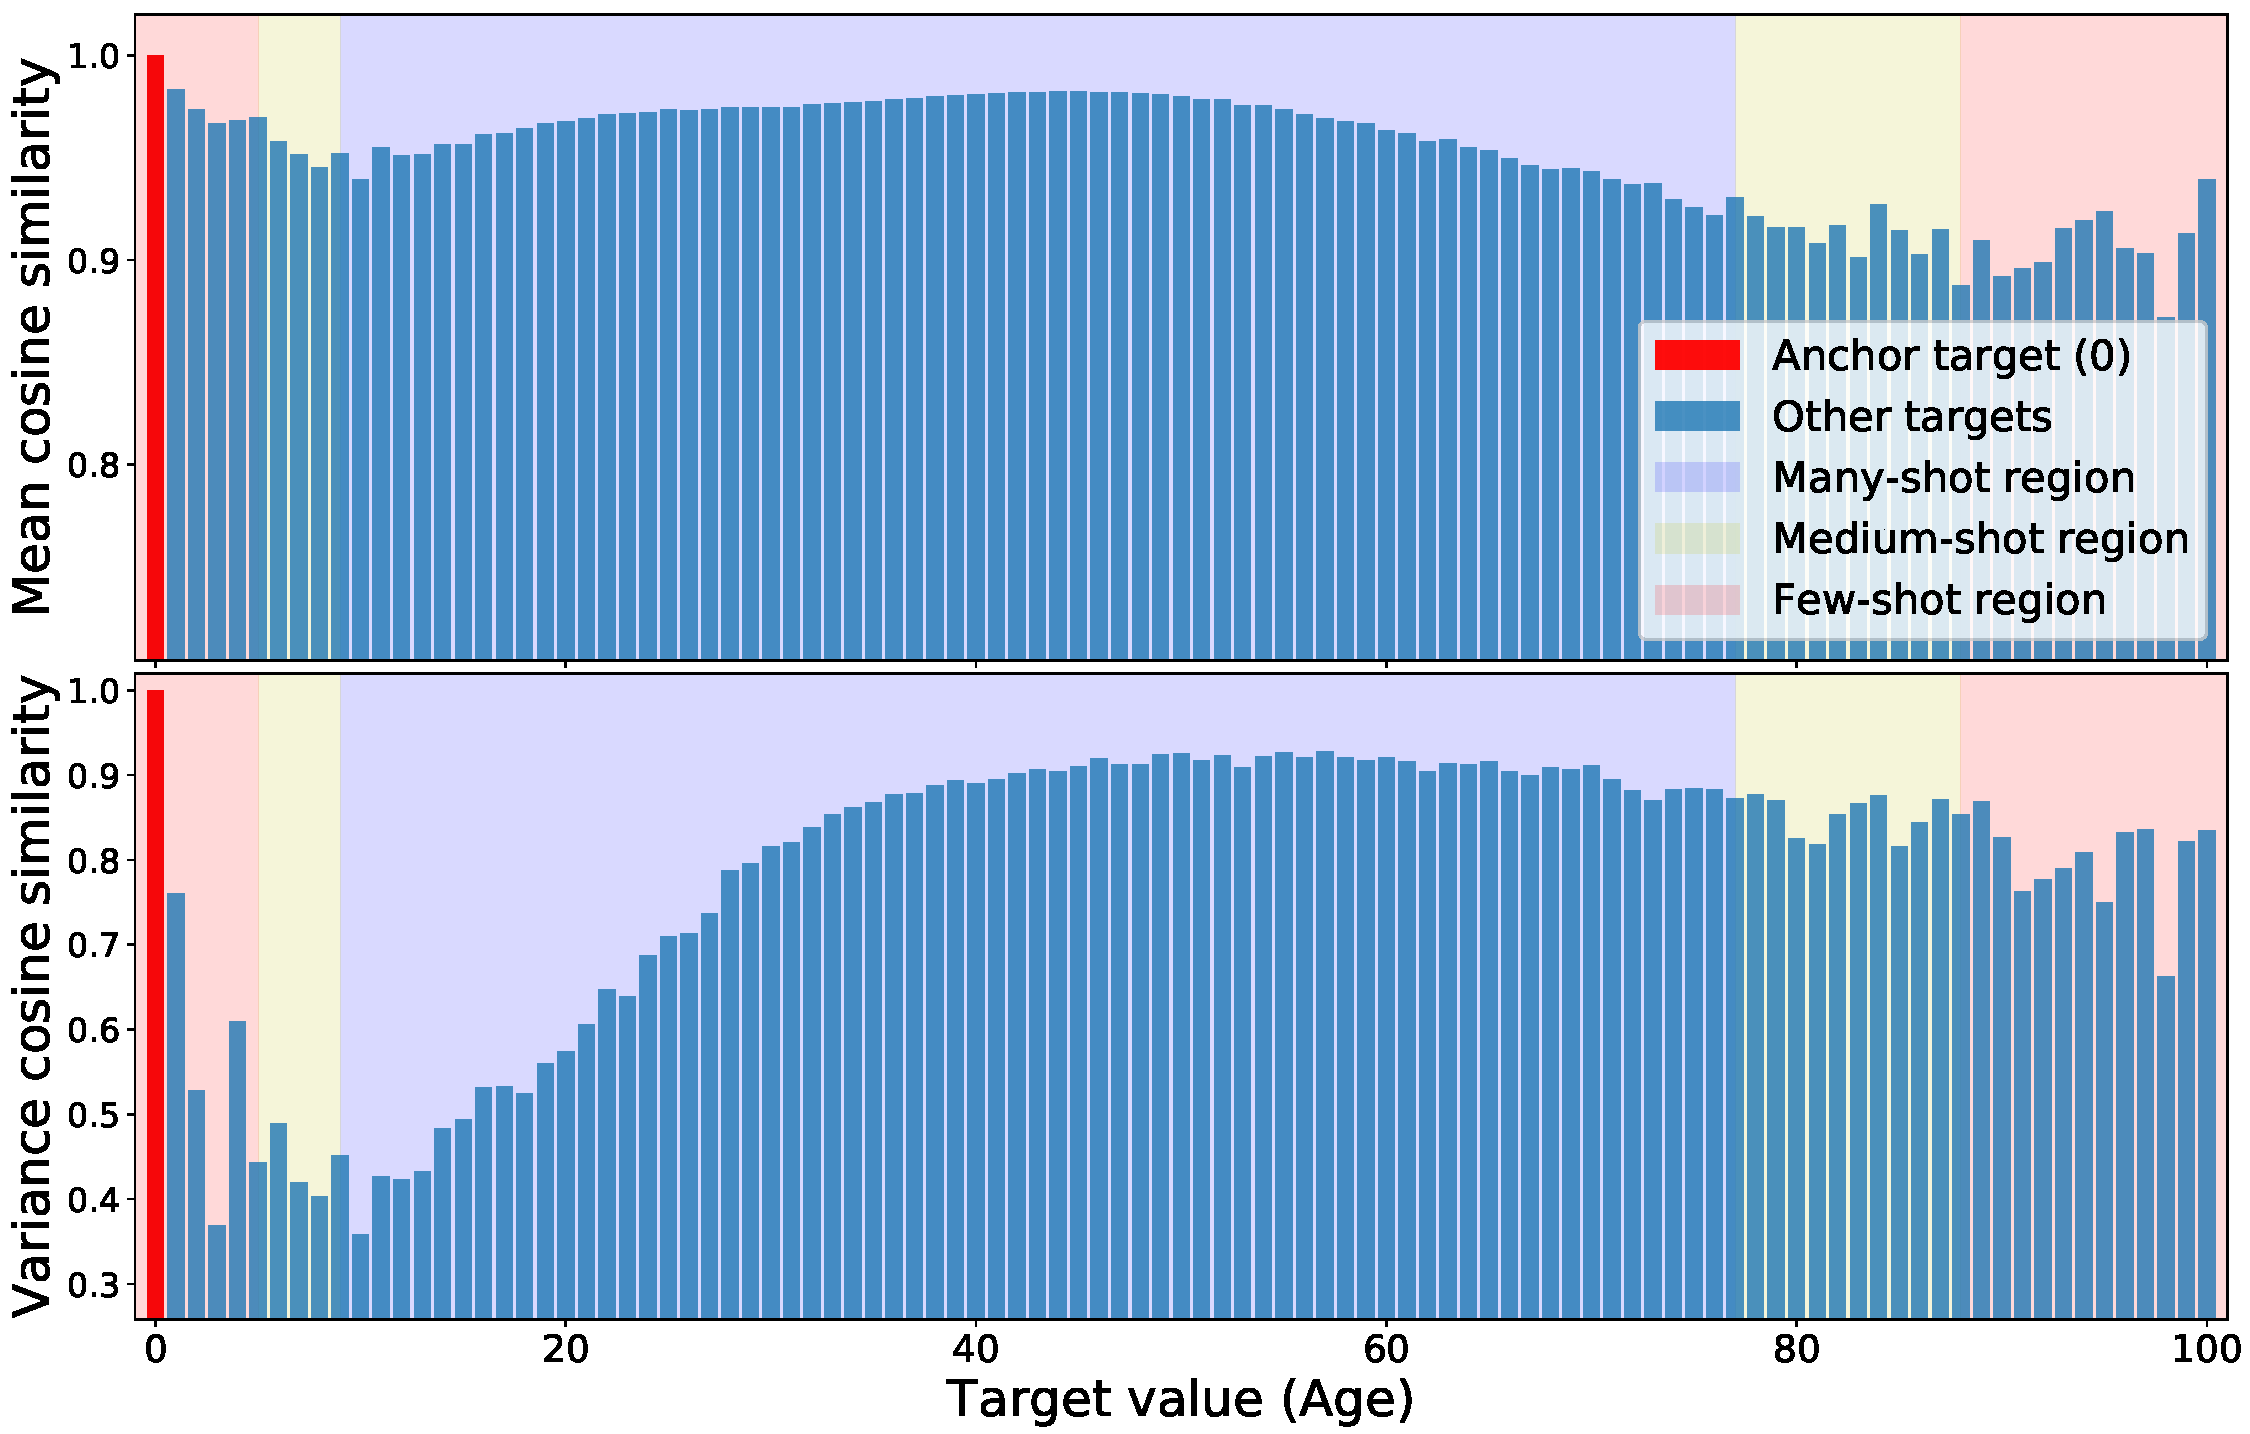
\includegraphics[width=\linewidth]{images/feat_sim_fds_base_0.pdf}
			\caption{Baseline}
		\end{subfigure}\hspace{1em}%
		\begin{subfigure}{0.48\textwidth}
			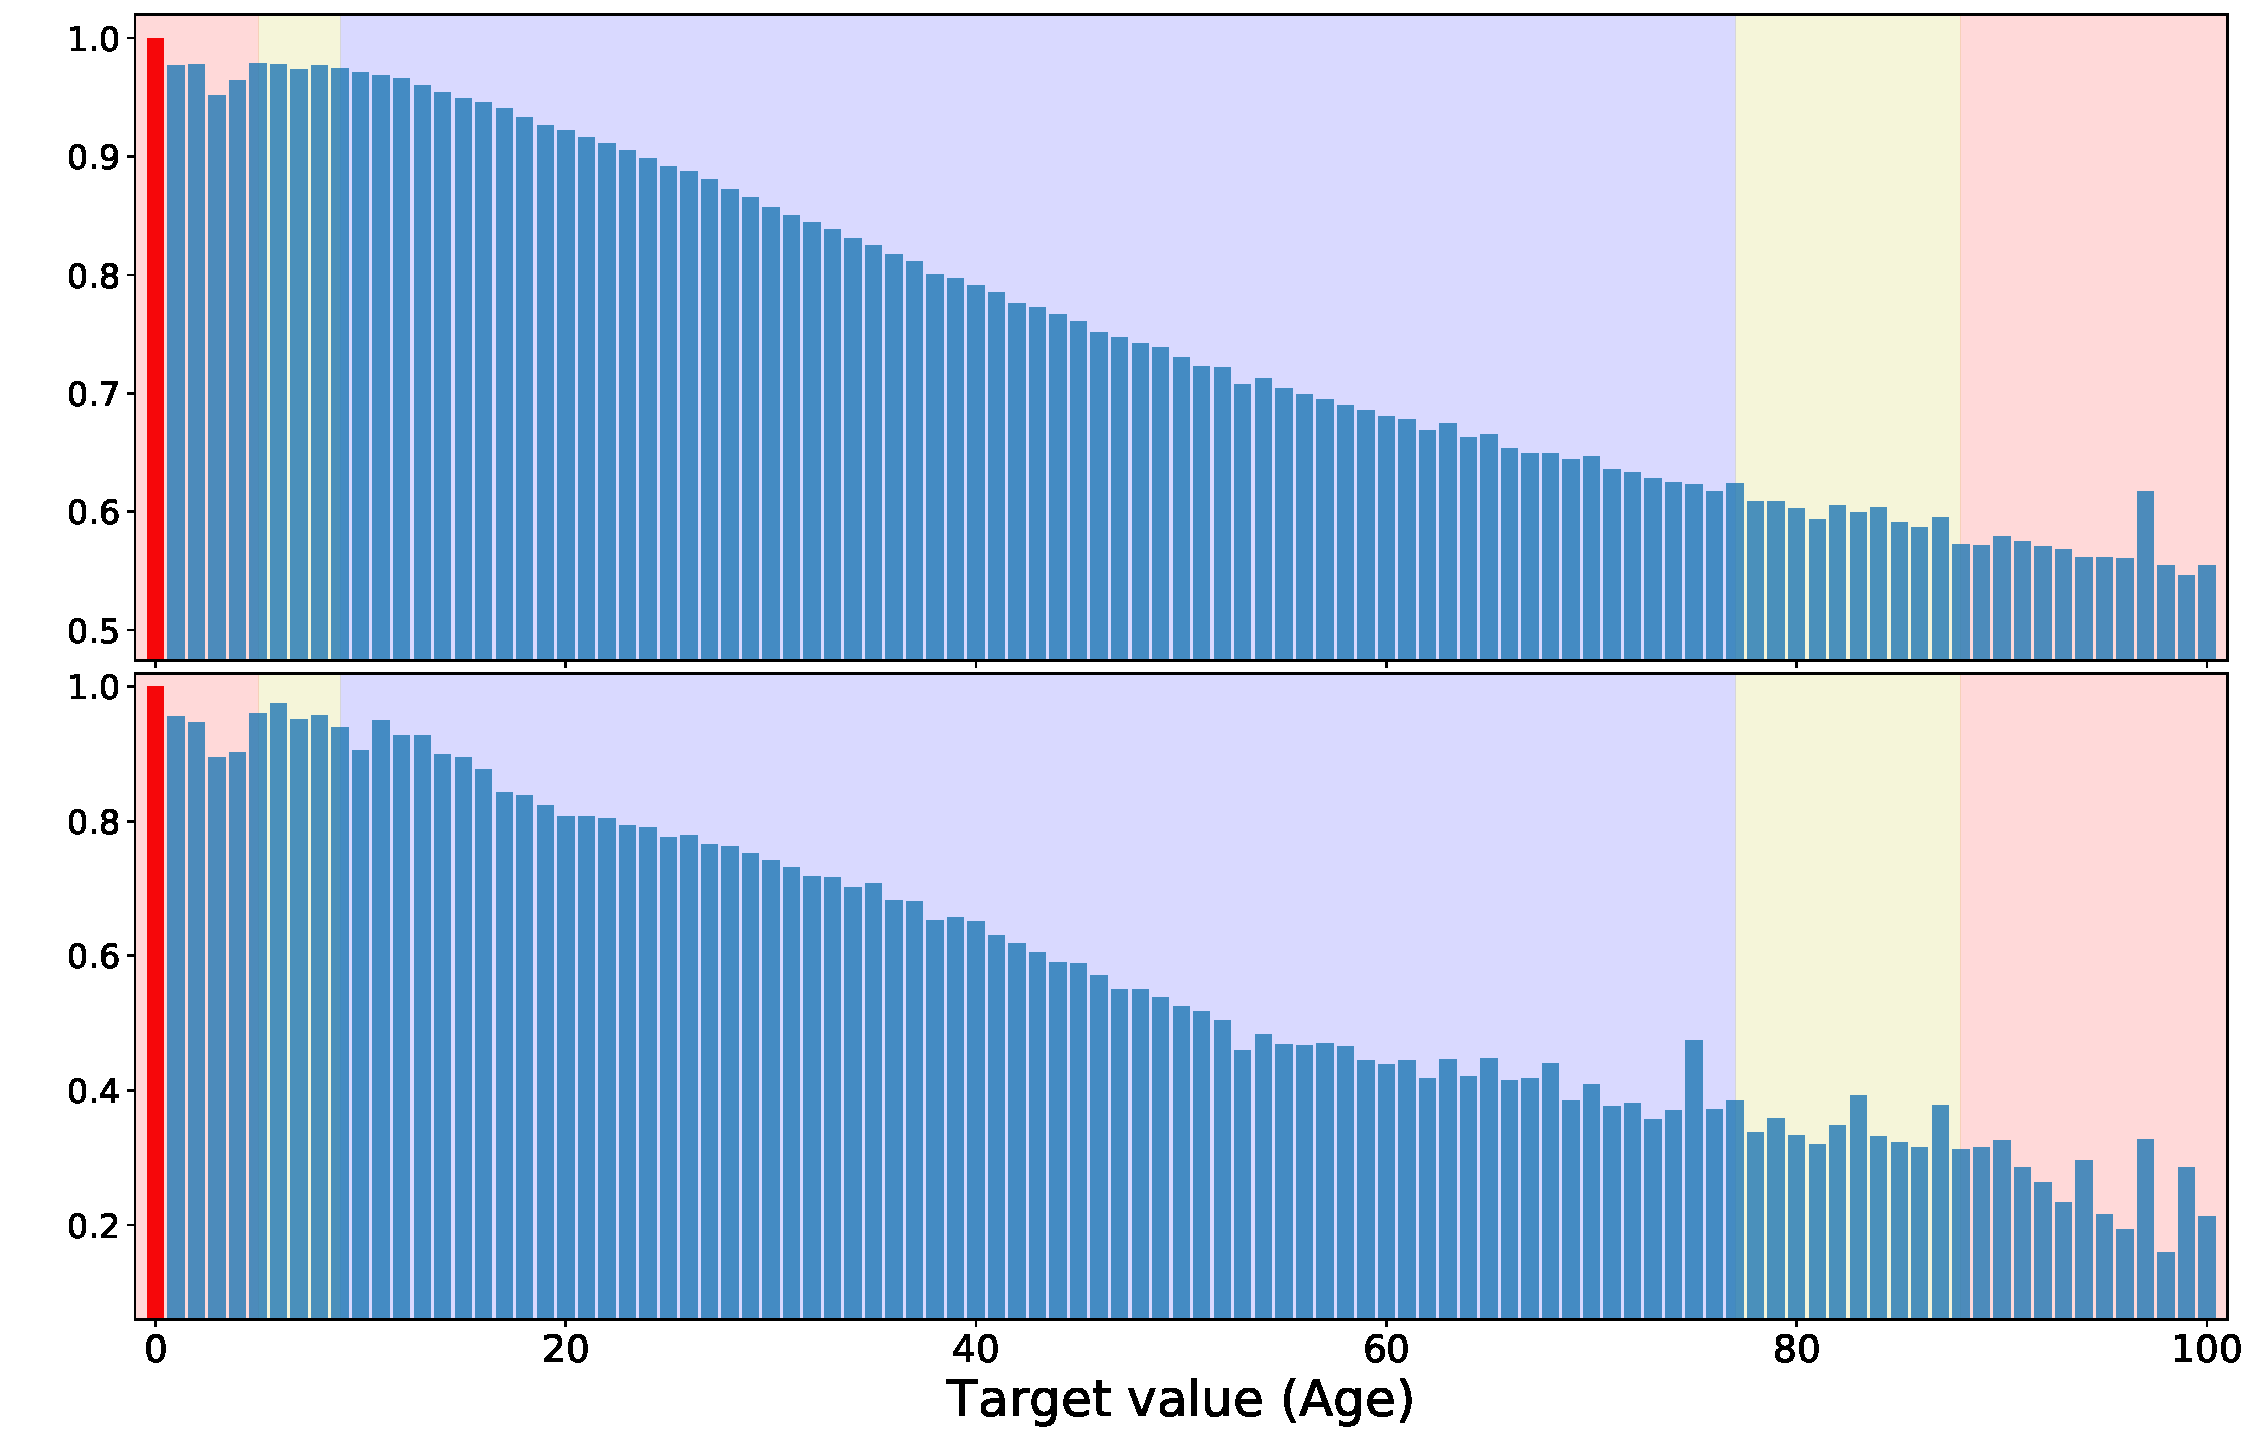
\includegraphics[width=\linewidth]{images/feat_sim_fds_ours_0.pdf}
			\caption{FDS}
		\end{subfigure}
		%\caption{}
	\end{figure}
	\begin{itemize}
		\item FDS improves feature statistics calibration:
		\begin{itemize}
			\item High similarity only in neighbourhood
			\item Gradually decreasing similarity as the target becomes smaller or larger
		\end{itemize}
	\end{itemize}
	\credit{Image}{yang2021delving}
\end{frame}

\begin{frame}{Feature statistics similarity for anchor age 30}
	\begin{figure}[h]
		\begin{subfigure}{0.48\textwidth}
			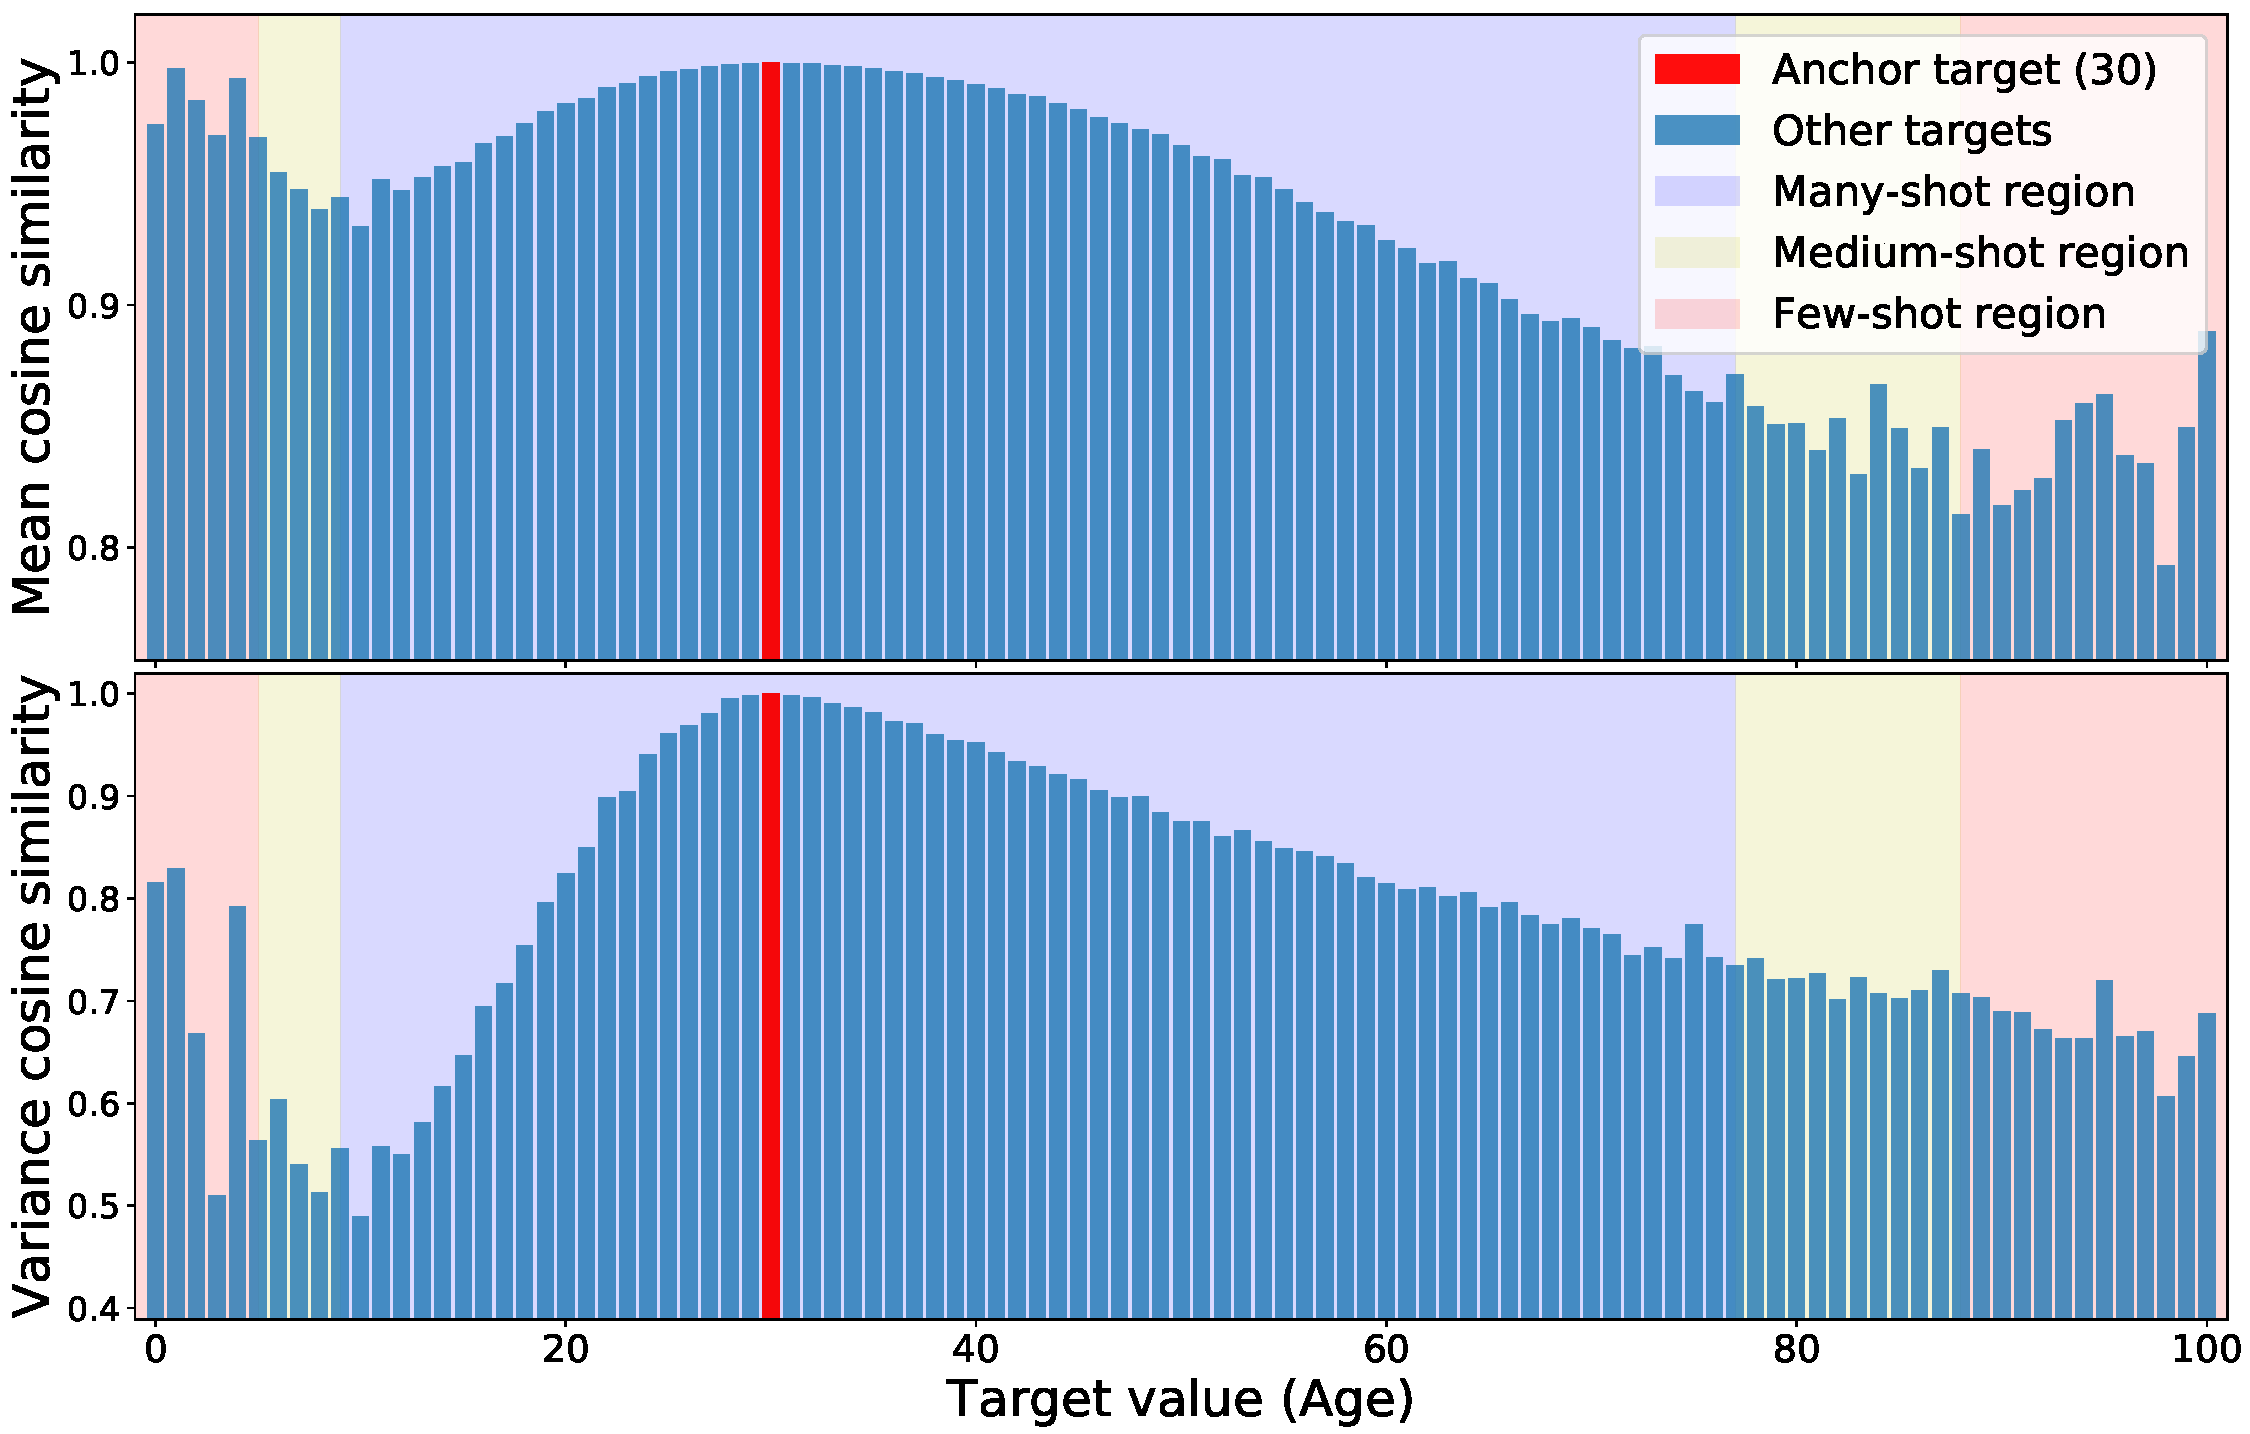
\includegraphics[width=\linewidth]{images/feat_sim_fds_base_30.pdf}
			\caption{Baseline}
		\end{subfigure}\hspace{1em}%
		\begin{subfigure}{0.48\textwidth}
			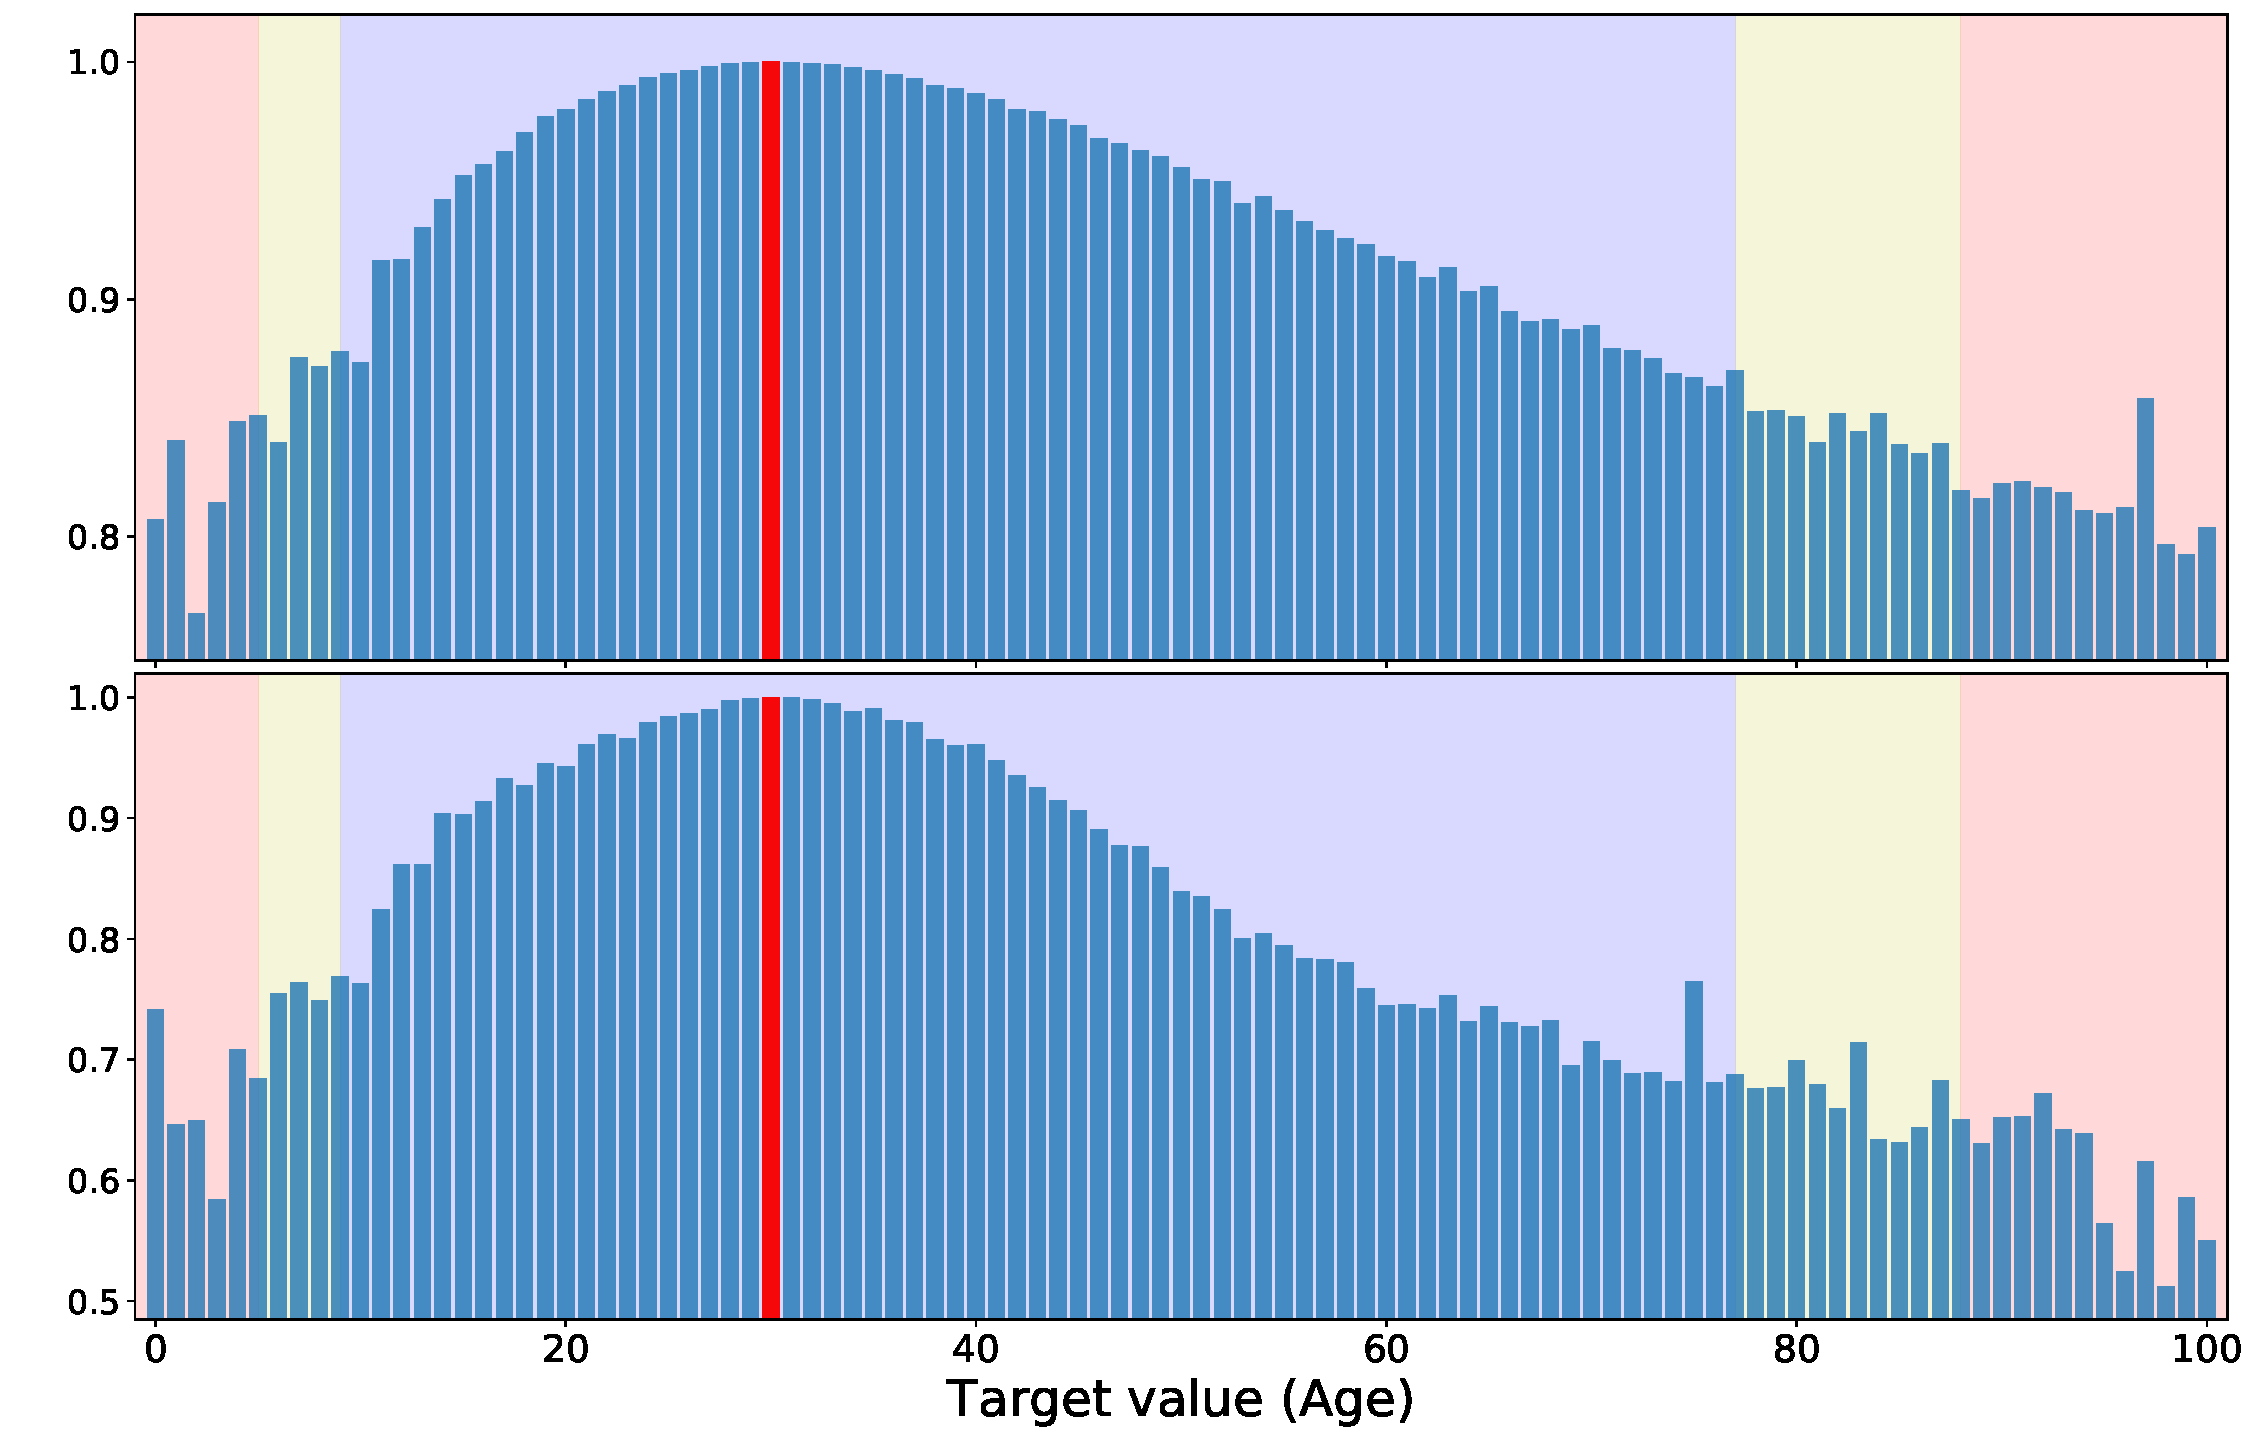
\includegraphics[width=\linewidth]{images/feat_sim_fds_ours_30.pdf}
			\caption{FDS}
		\end{subfigure}
		%\caption{}
	\end{figure}
	\begin{itemize}
		\item FDS improves feature statistics calibration:
		\begin{itemize}
			\item High similarity only in neighbourhood
			\item Gradually decreasing similarity as the target becomes smaller or larger
		\end{itemize}
	\end{itemize}
	\credit{Image}{yang2021delving}
\end{frame}

\begin{frame}{Feature statistics similarity for anchor age 60}
	\begin{figure}[h]
		\begin{subfigure}{0.48\textwidth}
			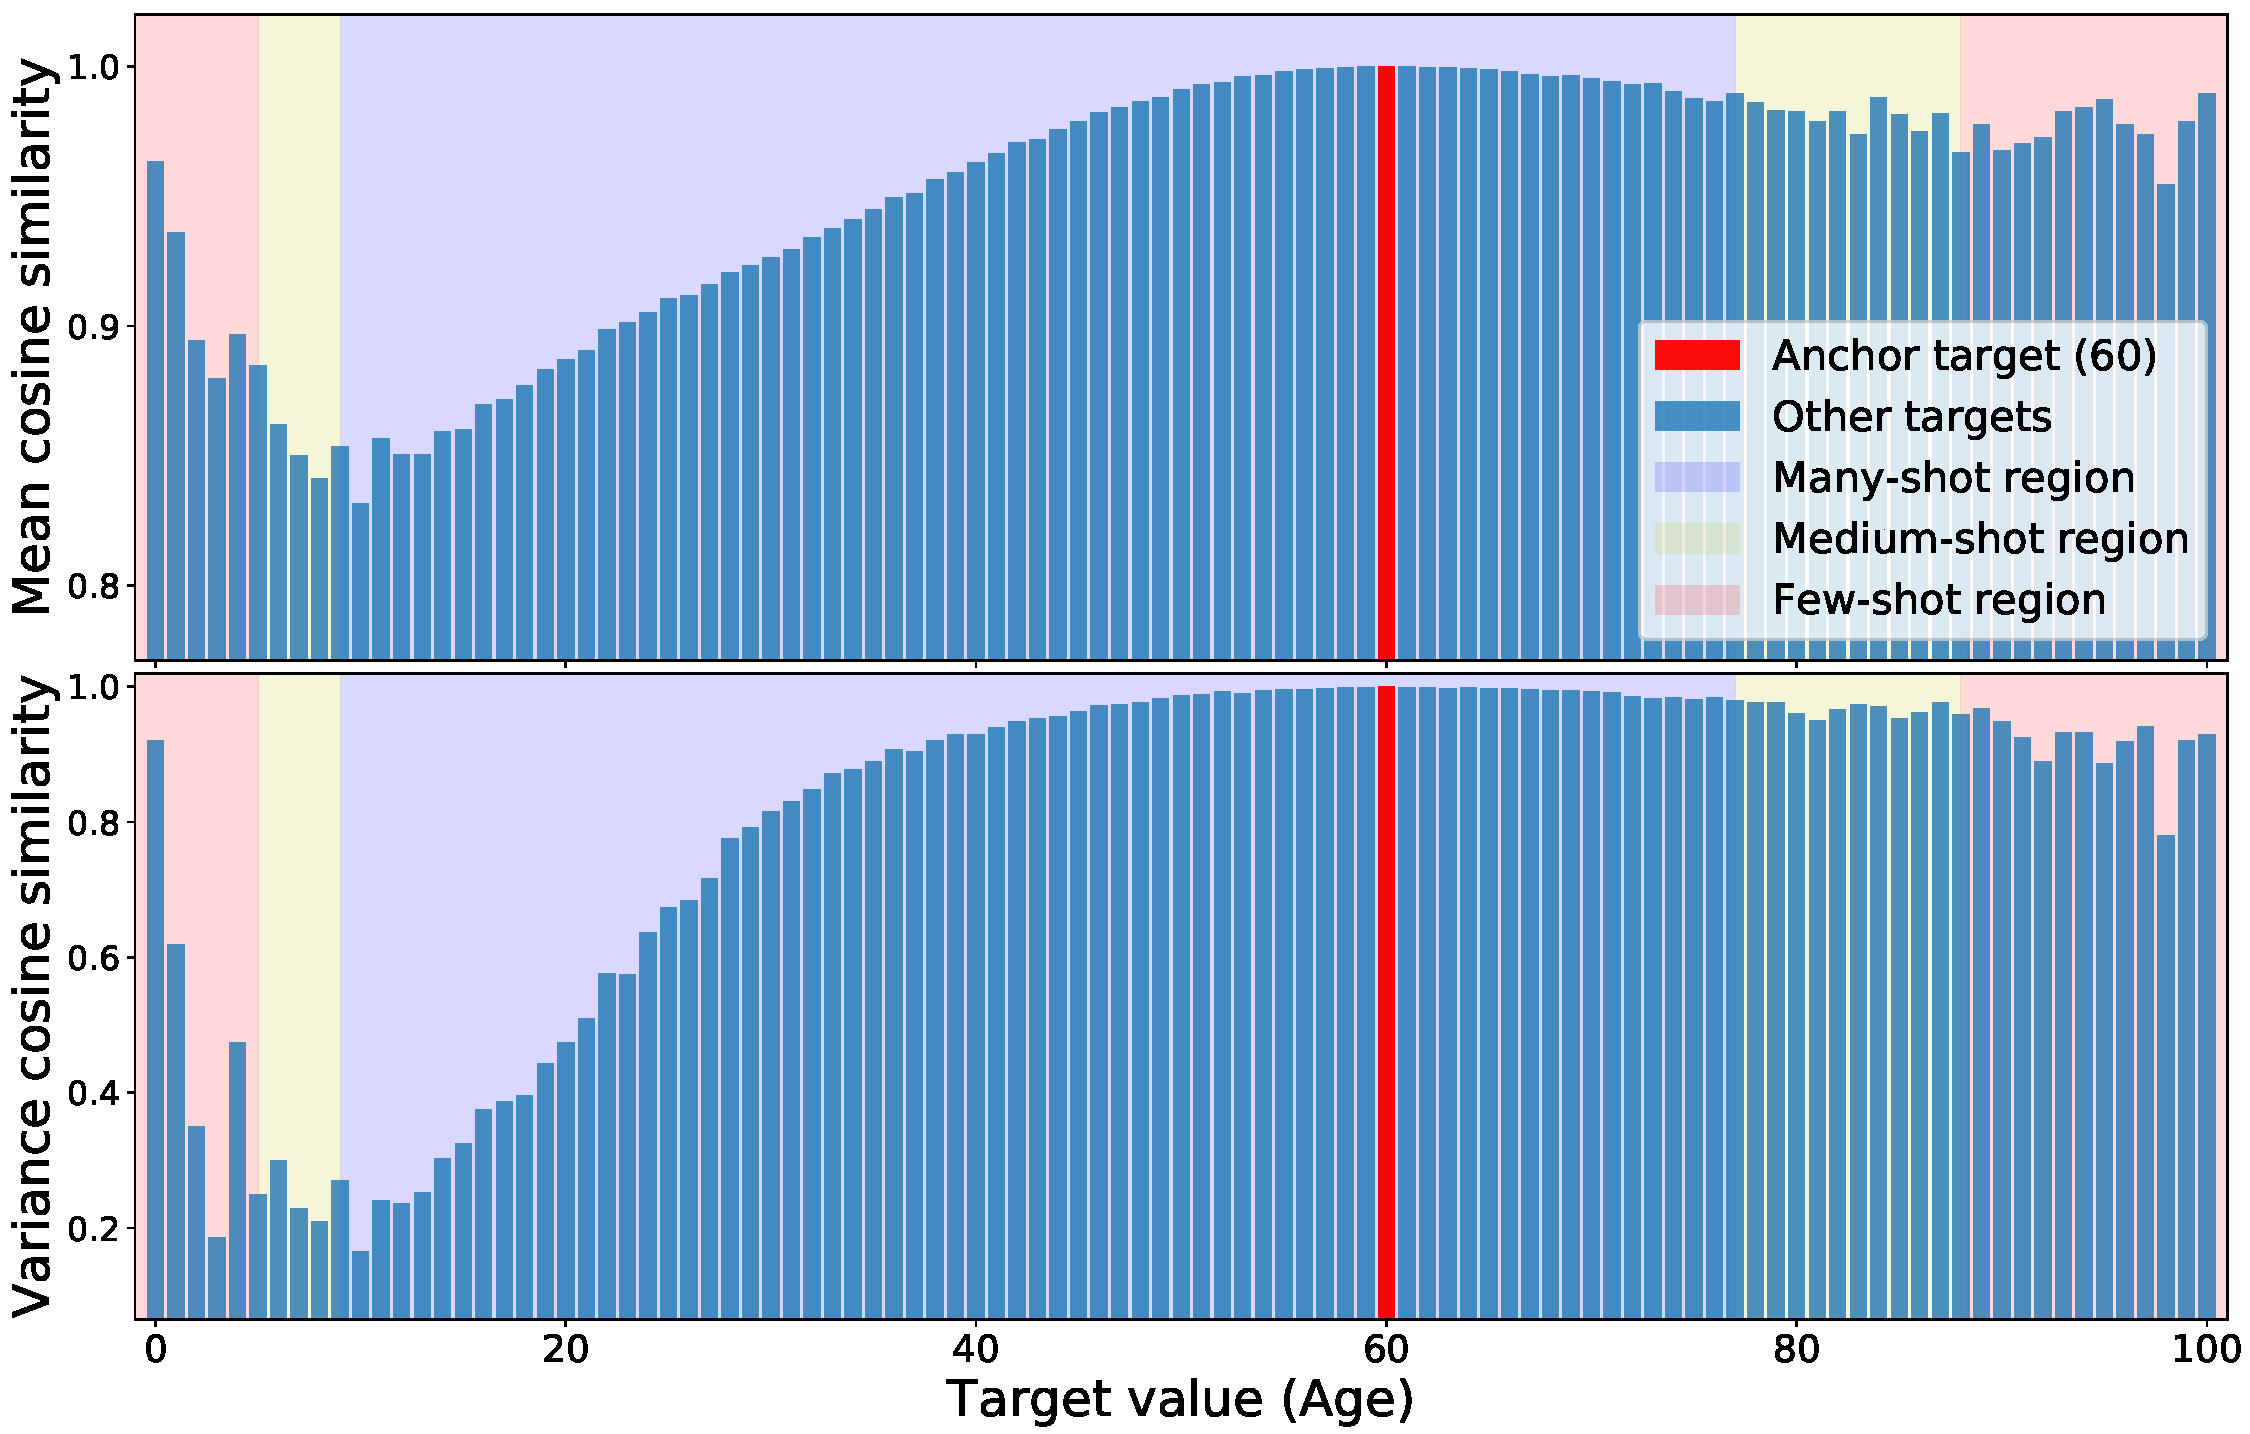
\includegraphics[width=\linewidth]{images/feat_sim_fds_base_60.pdf}
			\caption{Baseline}
		\end{subfigure}\hspace{1em}%
		\begin{subfigure}{0.48\textwidth}
			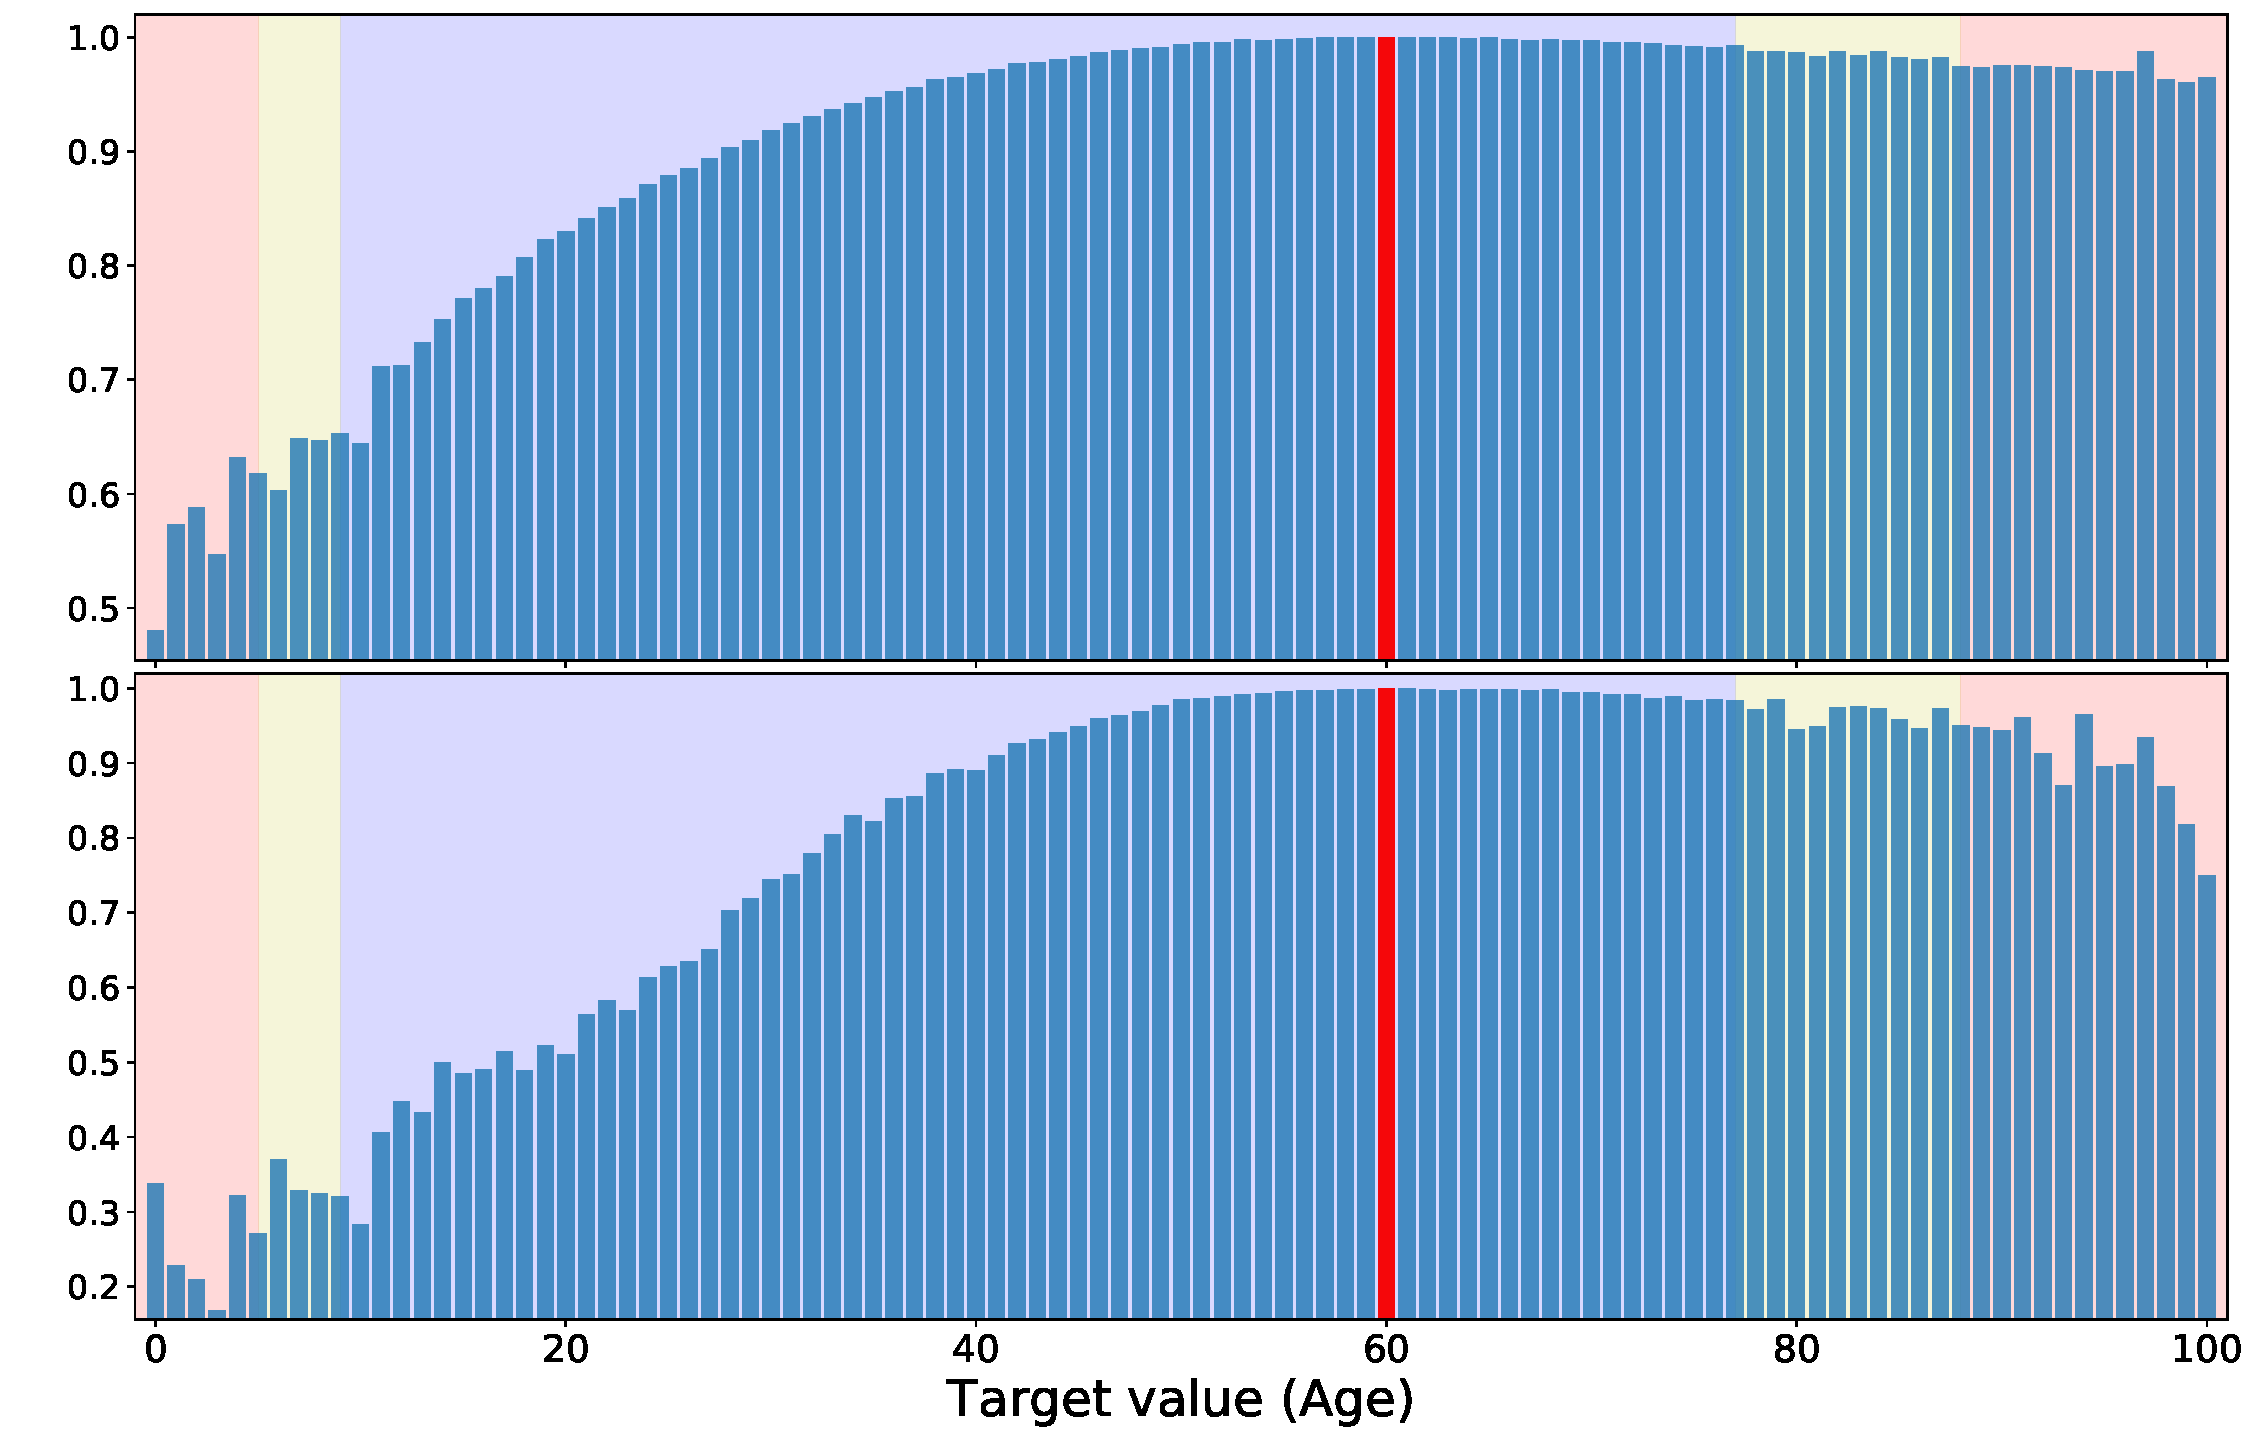
\includegraphics[width=\linewidth]{images/feat_sim_fds_ours_60.pdf}
			\caption{FDS}
		\end{subfigure}
		%\caption{}
	\end{figure}
	\begin{itemize}
		\item FDS improves feature statistics calibration:
		\begin{itemize}
			\item High similarity only in neighbourhood
			\item Gradually decreasing similarity as the target becomes smaller or larger
		\end{itemize}
	\end{itemize}
	\credit{Image}{yang2021delving}
\end{frame}

\begin{frame}{Feature statistics similarity for anchor age 90}
	\begin{figure}[h]
		\begin{subfigure}{0.48\textwidth}
			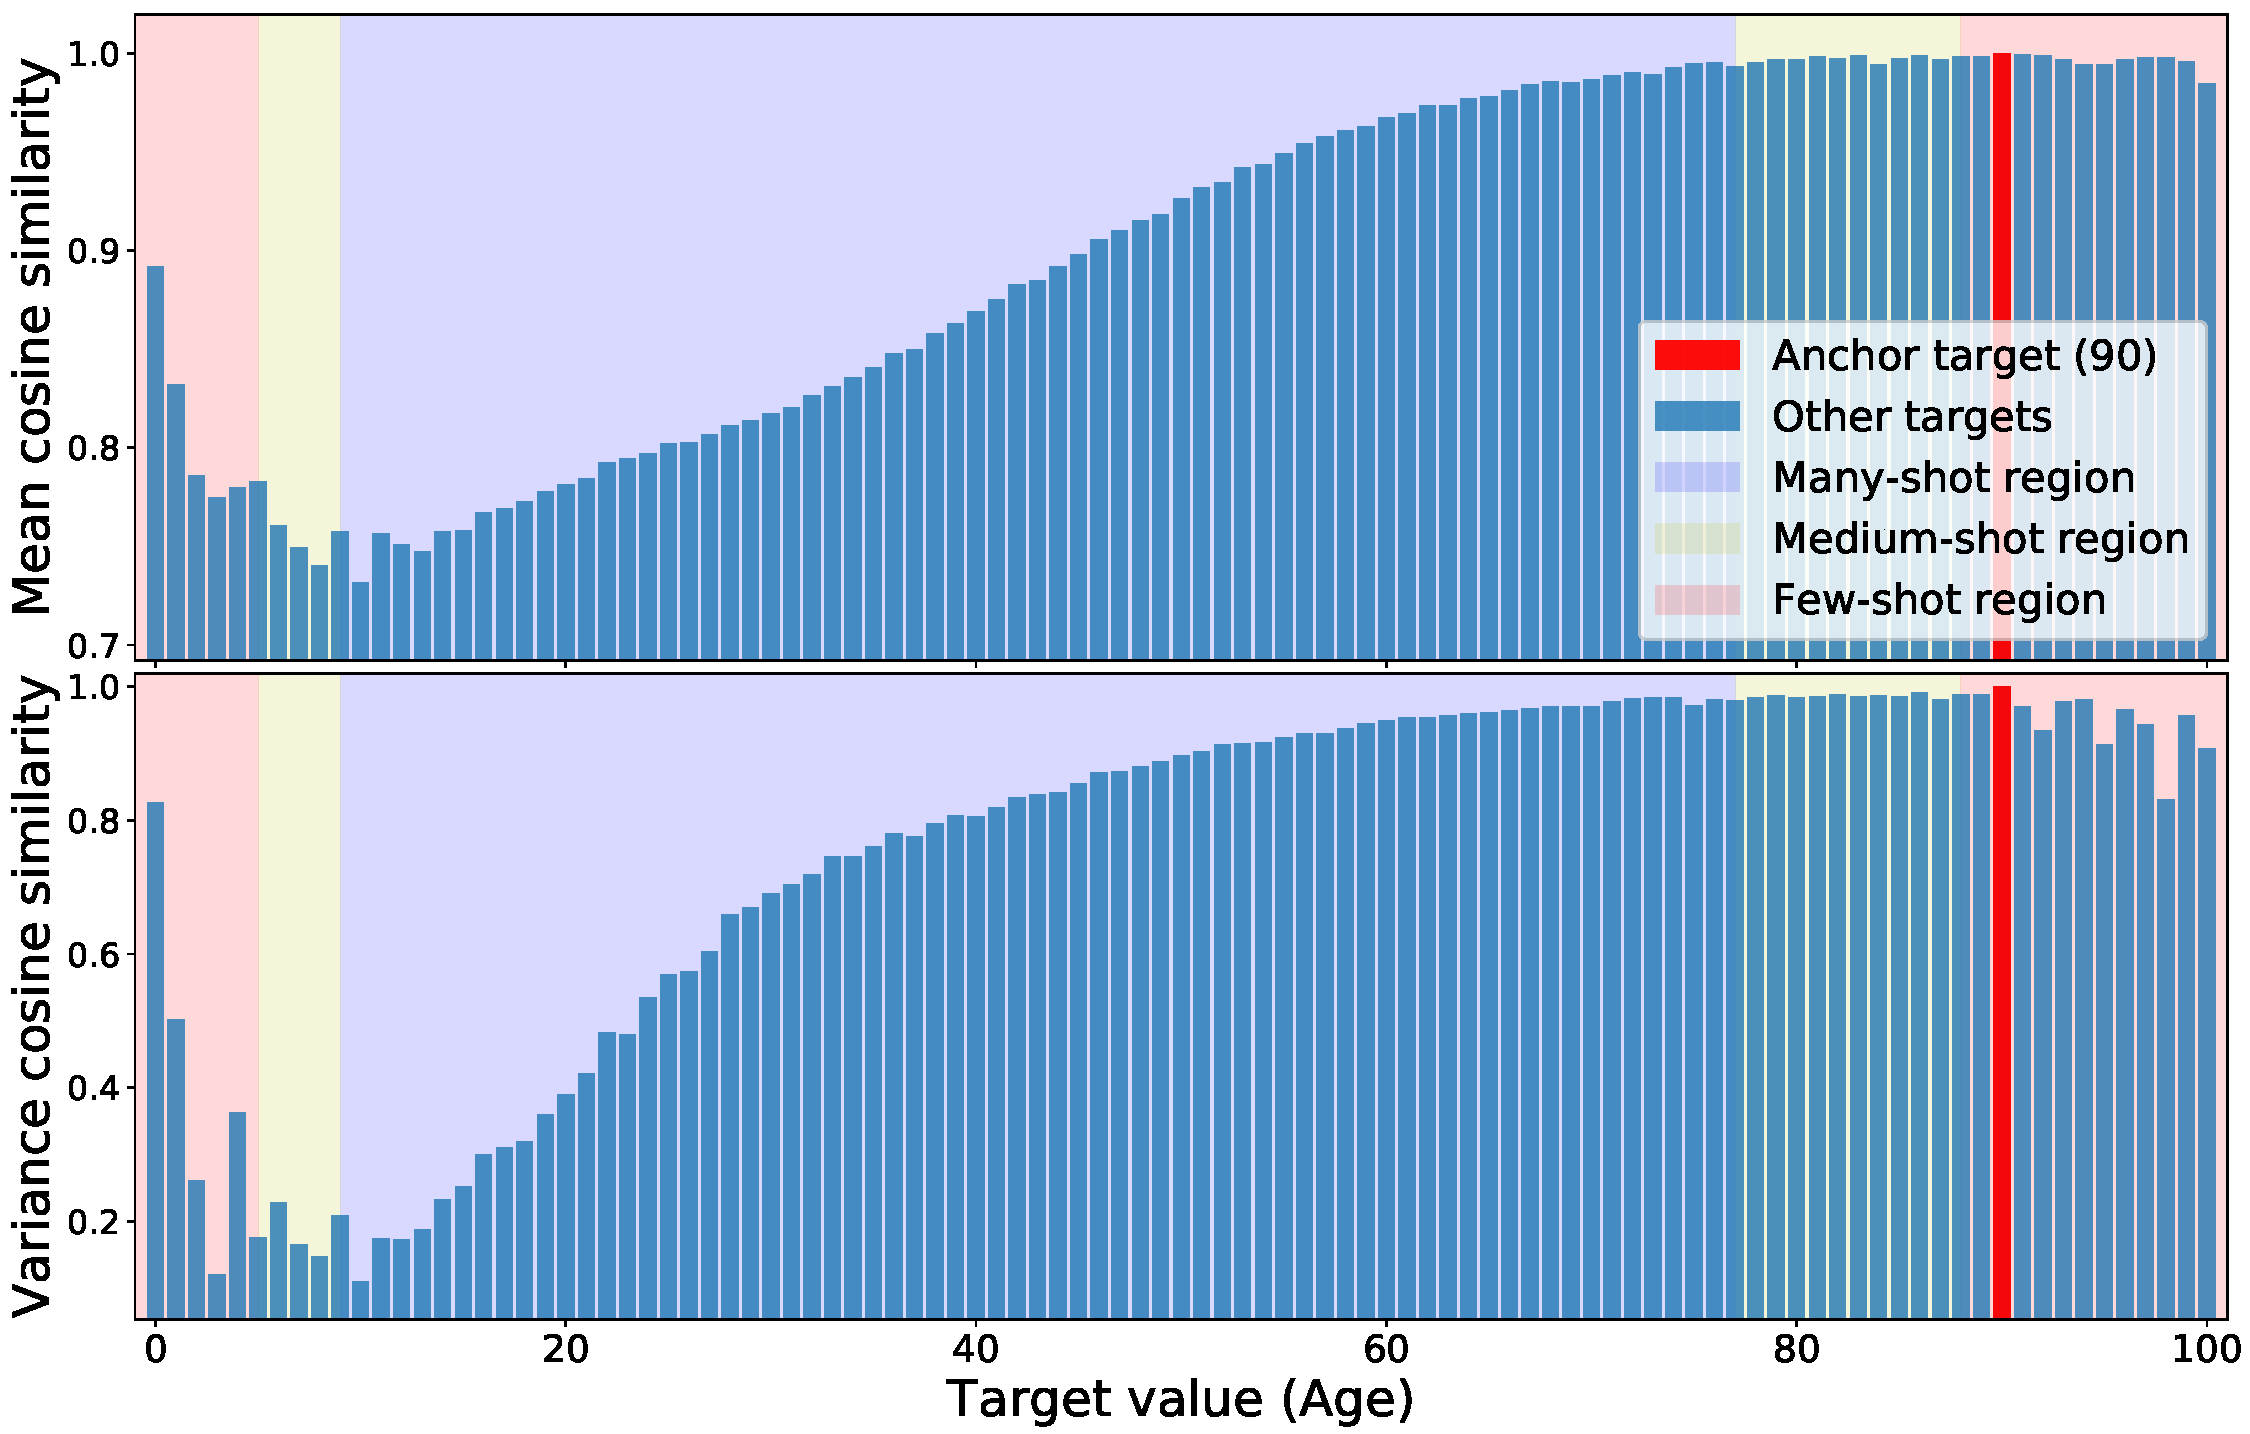
\includegraphics[width=\linewidth]{images/feat_sim_fds_base_90.pdf}
			\caption{Baseline}
		\end{subfigure}\hspace{1em}%
		\begin{subfigure}{0.48\textwidth}
			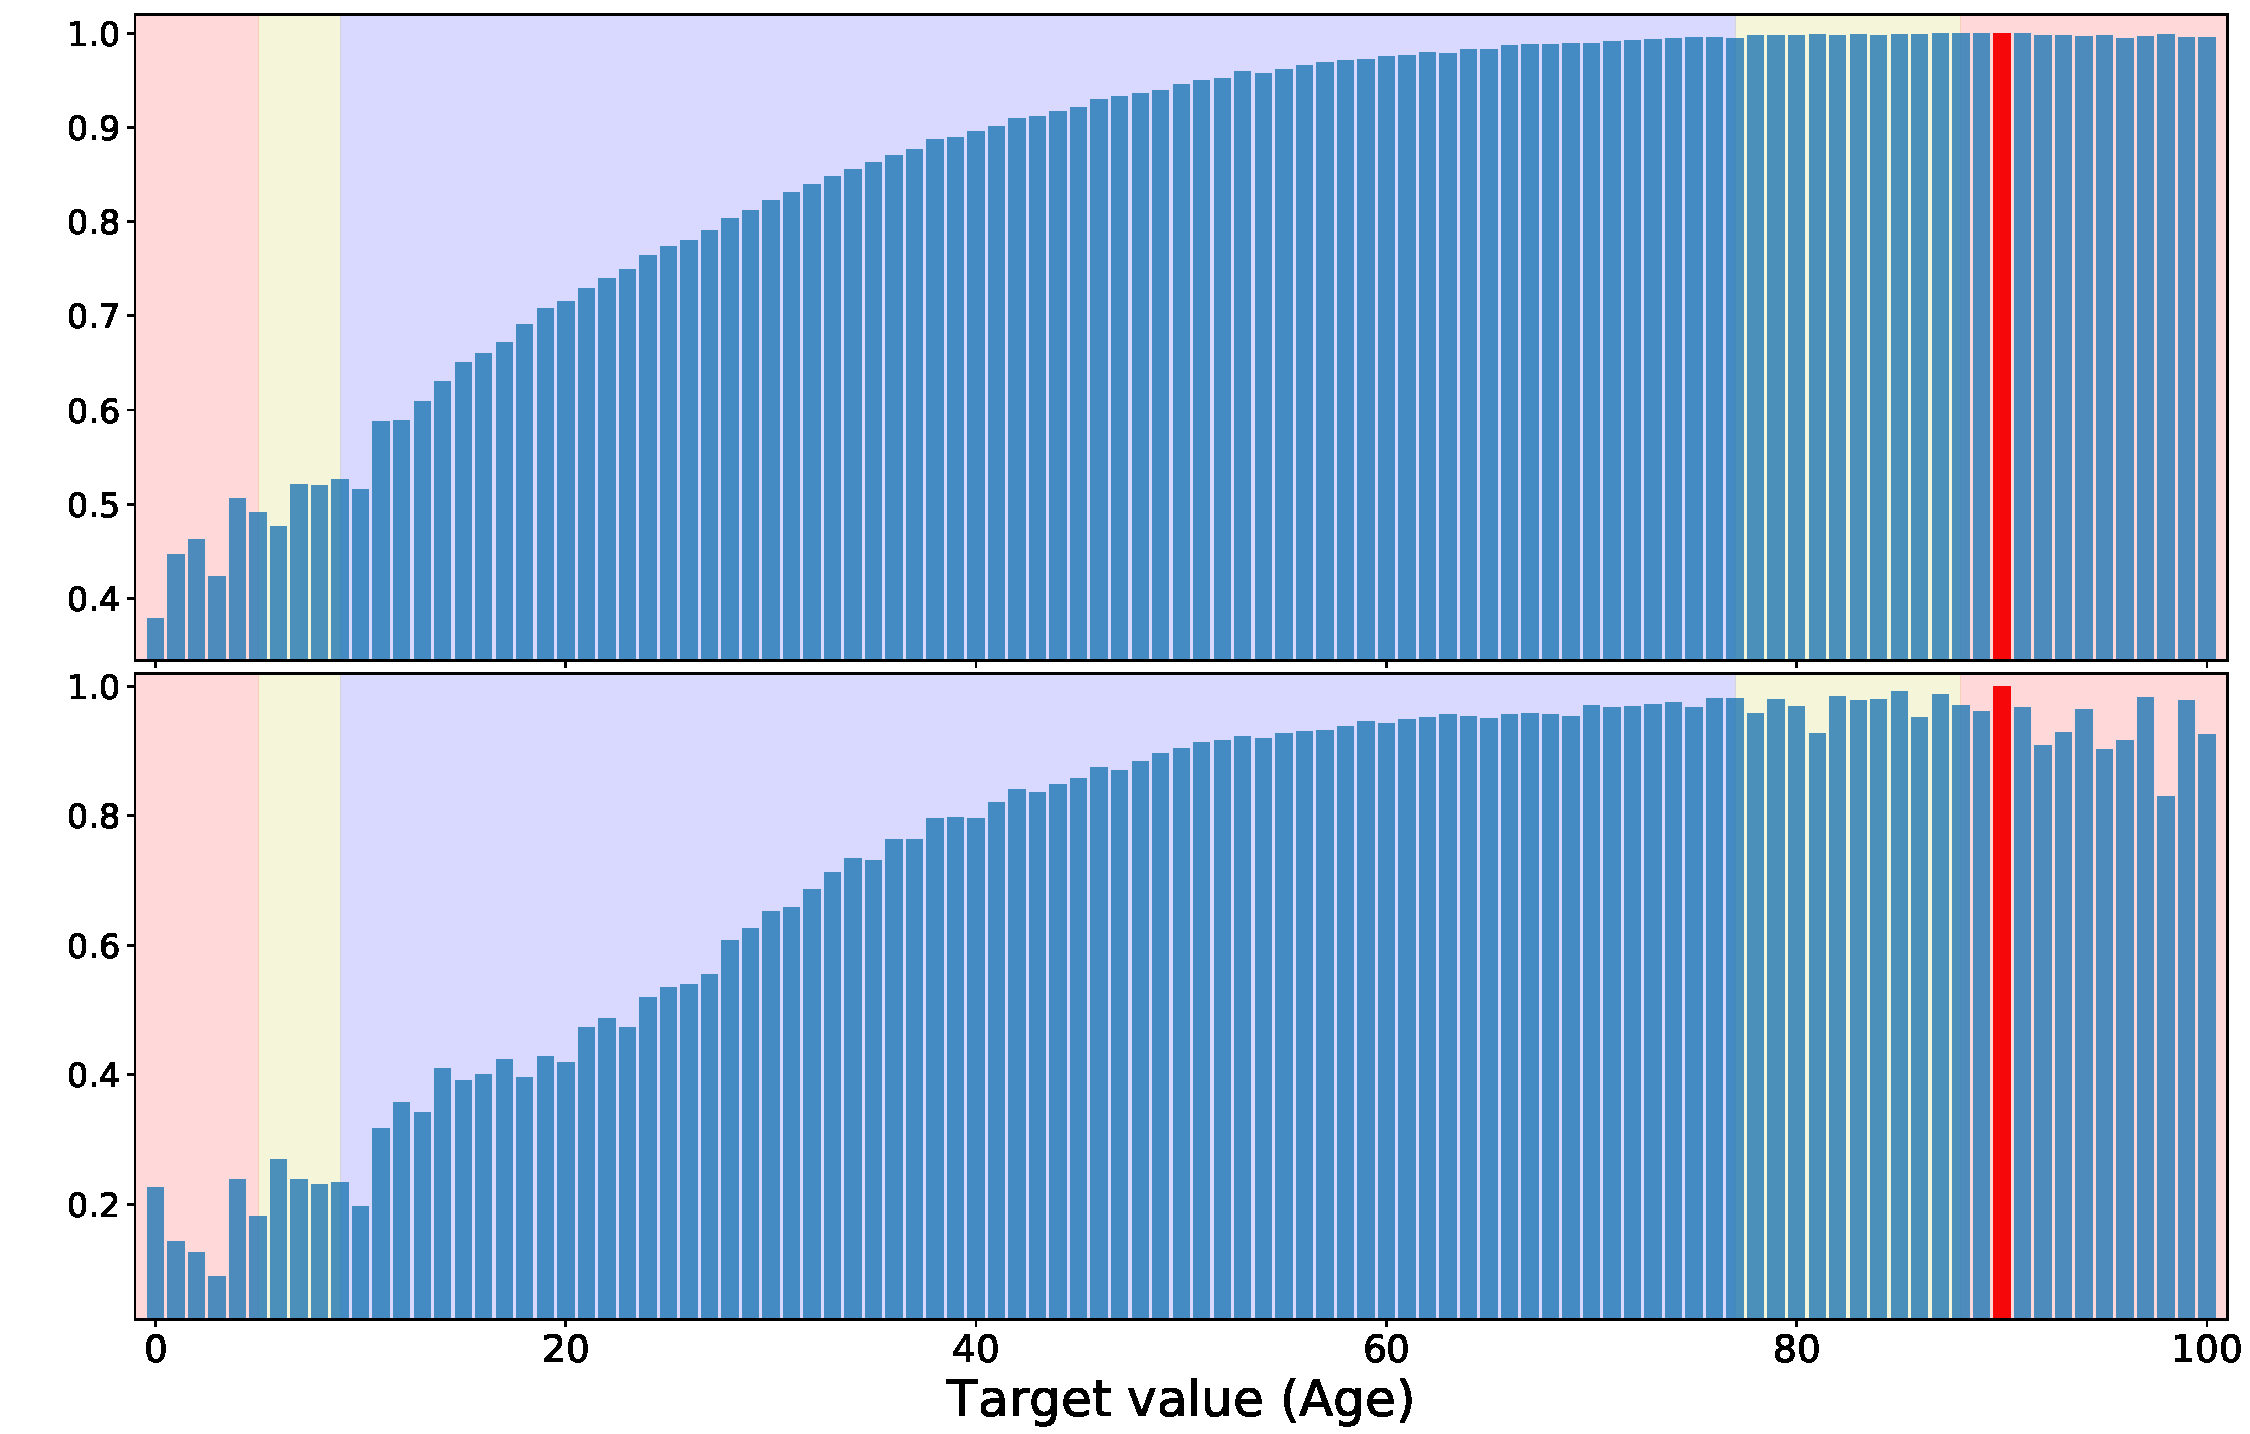
\includegraphics[width=\linewidth]{images/feat_sim_fds_ours_90.pdf}
			\caption{FDS}
		\end{subfigure}
		%\caption{}
	\end{figure}
	\begin{itemize}
		\item FDS improves feature statistics calibration:
		\begin{itemize}
			\item High similarity only in neighbourhood
			\item Gradually decreasing similarity as the target becomes smaller or larger
		\end{itemize}
	\end{itemize}
	\credit{Image}{yang2021delving}
\end{frame}

\begin{frame}{The FDS Algorithm}
	\begin{figure}[h]
		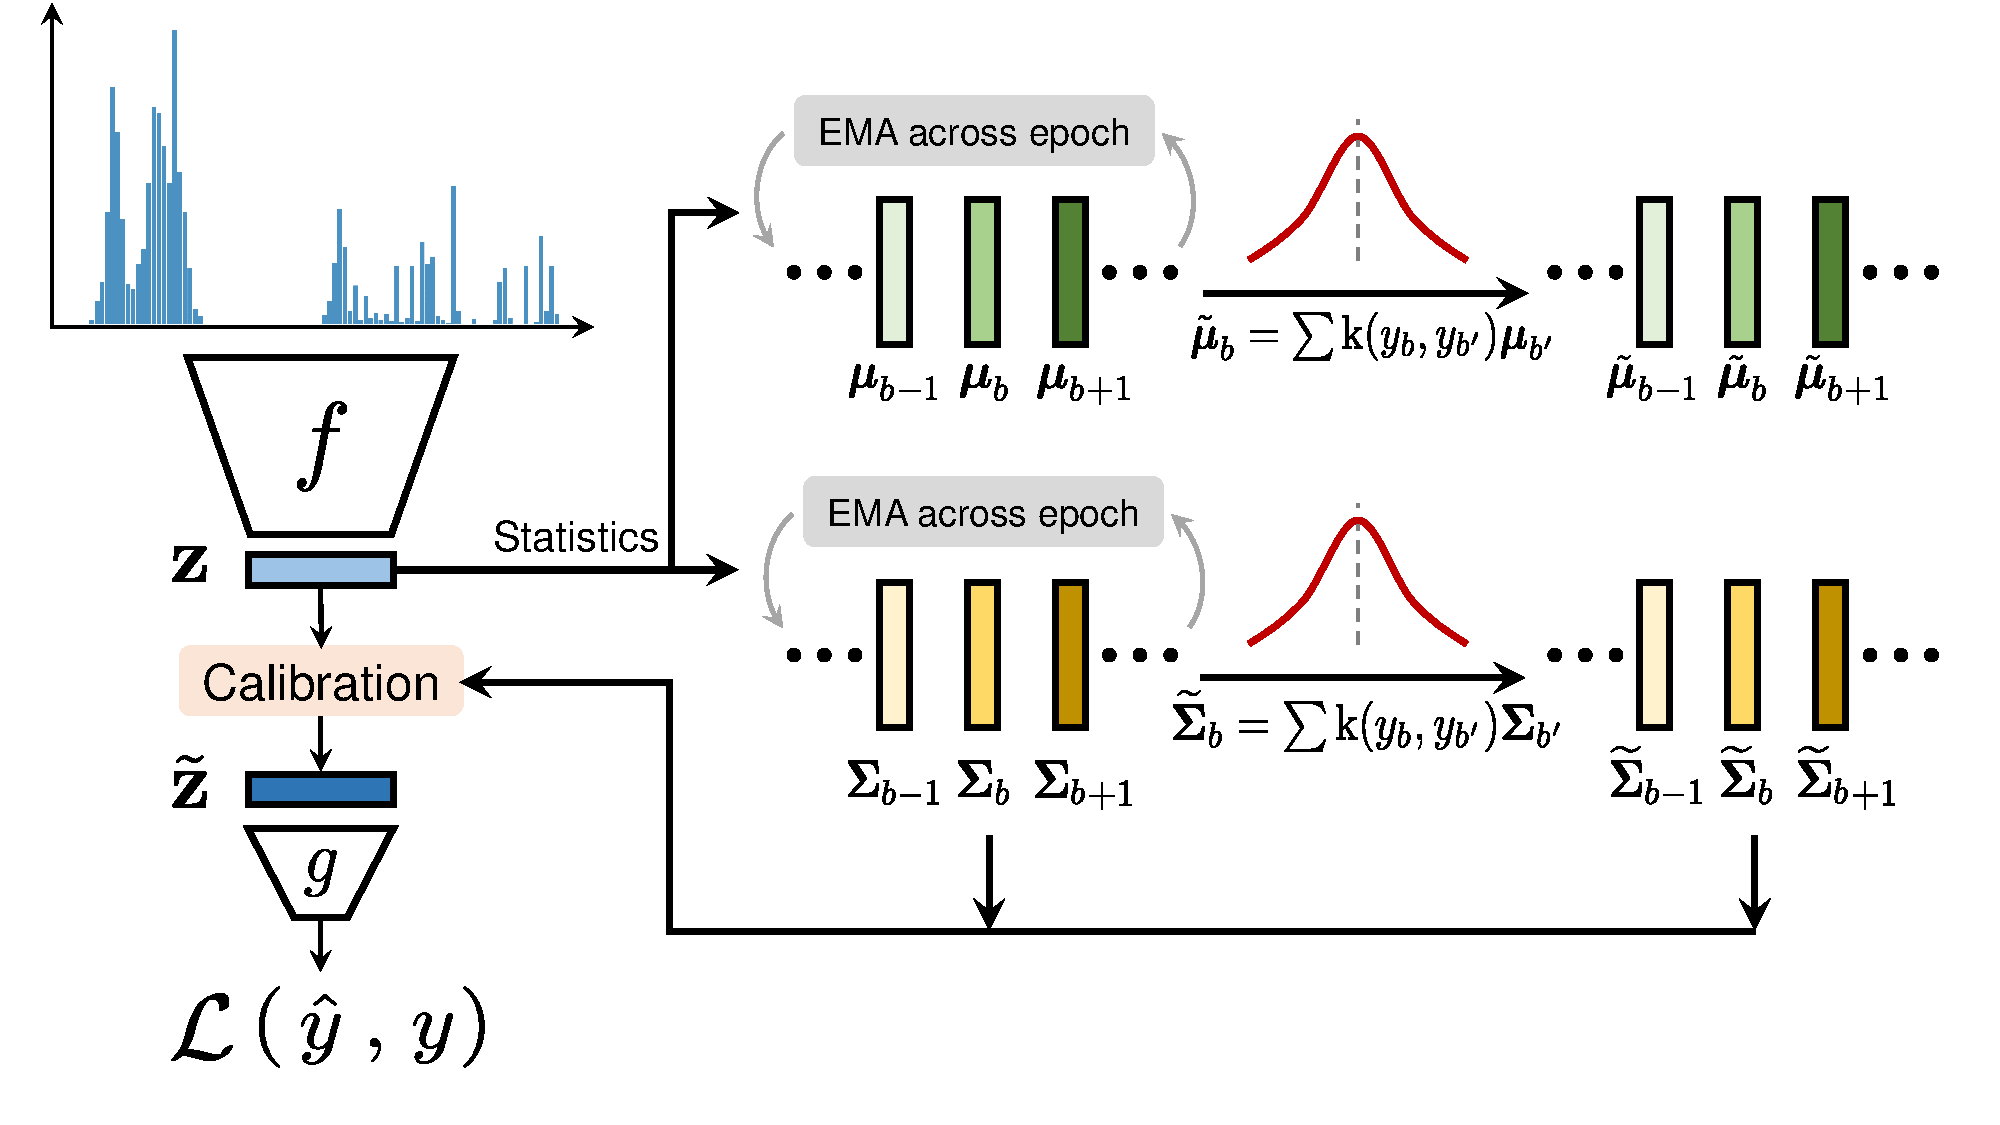
\includegraphics[width=\linewidth]{images/teaser_fds.pdf}
		%\caption{}
	\end{figure}
	\credit{Image}{yang2021delving}
\end{frame}